% This file is generated by the MATLAB m-file laprint.m. It can be included
% into LaTeX documents using the packages epsfig and psfrag. It is accompanied
% by a postscript file. A sample LaTeX file is:
%    \documentclass{article} \usepackage{epsfig,psfrag}
%    \begin{document}\begin{figure}% This file is generated by the MATLAB m-file laprint.m. It can be included
% into LaTeX documents using the packages epsfig and psfrag. It is accompanied
% by a postscript file. A sample LaTeX file is:
%    \documentclass{article} \usepackage{epsfig,psfrag}
%    \begin{document}\begin{figure}% This file is generated by the MATLAB m-file laprint.m. It can be included
% into LaTeX documents using the packages epsfig and psfrag. It is accompanied
% by a postscript file. A sample LaTeX file is:
%    \documentclass{article} \usepackage{epsfig,psfrag}
%    \begin{document}\begin{figure}% This file is generated by the MATLAB m-file laprint.m. It can be included
% into LaTeX documents using the packages epsfig and psfrag. It is accompanied
% by a postscript file. A sample LaTeX file is:
%    \documentclass{article} \usepackage{epsfig,psfrag}
%    \begin{document}\begin{figure}\input{energy}\end{figure}\end{document}
% See http://www.uni-kassel.de/~linne/ for recent versions of laprint.m.
%
% created by:           LaPrint version 2.03 (19.1.2000)
% created on:           06-Oct-2009 10:58:03
% options used:         / noextrapicture
% latex width:          12 cm
% factor:               0.8
% eps file name:        energy.eps
% eps bounding box:     15 cm x 11.25 cm
% comment:              
%
\begin{psfrags}%
\psfragscanon%
%
% text strings:
\psfrag{str01}[t][t]{\sf Time (days)}%
\psfrag{str02}[t][t]{\sf Energy price}%
%
% xticklabels:
\psfrag{x01}[t][t]{0}%
\psfrag{x02}[t][t]{\sf 100}%
\psfrag{x03}[t][t]{\sf 200}%
\psfrag{x04}[t][t]{\sf 300}%
\psfrag{x05}[t][t]{\sf 400}%
\psfrag{x06}[t][t]{\sf 500}%
\psfrag{x07}[t][t]{\sf 600}%
%
% yticklabels:
\psfrag{v01}[r][r]{}%
\psfrag{v02}[r][r]{\sf $p_0$}%
\psfrag{v03}[r][r]{\sf $(1+\pi) p_0$}%
\psfrag{v04}[r][r]{\sf $(1+\pi)^2 p_0$}%
\psfrag{v05}[r][r]{}%
\psfrag{v06}[r][r]{}%
\psfrag{v07}[r][r]{}%
\psfrag{v08}[r][r]{}%
\psfrag{v09}[r][r]{}%
%
% Figure:
\resizebox{12cm}{!}{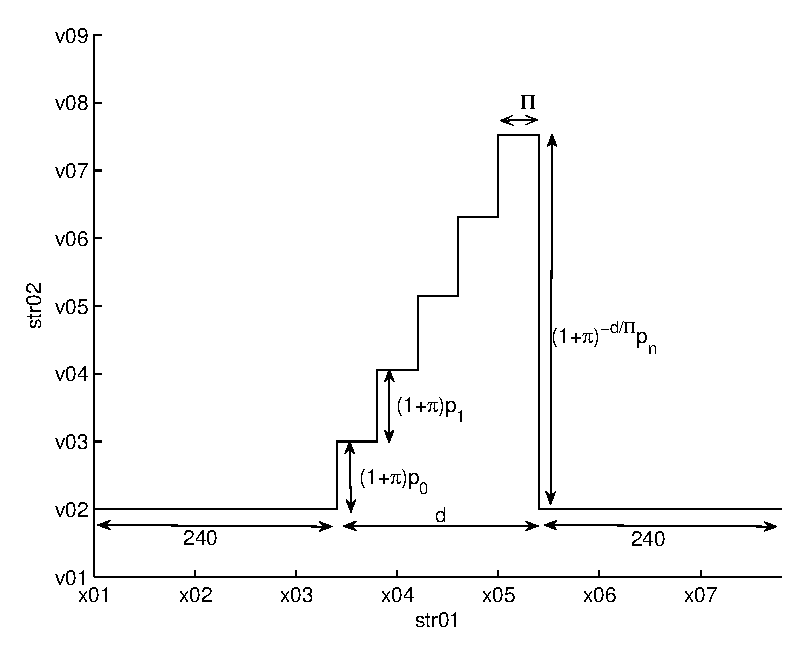
\epsfig{file=./energy_shock/eps/energy.eps}}%
\end{psfrags}%
%
% End energy.tex
\end{figure}\end{document}
% See http://www.uni-kassel.de/~linne/ for recent versions of laprint.m.
%
% created by:           LaPrint version 2.03 (19.1.2000)
% created on:           06-Oct-2009 10:58:03
% options used:         / noextrapicture
% latex width:          12 cm
% factor:               0.8
% eps file name:        energy.eps
% eps bounding box:     15 cm x 11.25 cm
% comment:              
%
\begin{psfrags}%
\psfragscanon%
%
% text strings:
\psfrag{str01}[t][t]{\sf Time (days)}%
\psfrag{str02}[t][t]{\sf Energy price}%
%
% xticklabels:
\psfrag{x01}[t][t]{0}%
\psfrag{x02}[t][t]{\sf 100}%
\psfrag{x03}[t][t]{\sf 200}%
\psfrag{x04}[t][t]{\sf 300}%
\psfrag{x05}[t][t]{\sf 400}%
\psfrag{x06}[t][t]{\sf 500}%
\psfrag{x07}[t][t]{\sf 600}%
%
% yticklabels:
\psfrag{v01}[r][r]{}%
\psfrag{v02}[r][r]{\sf $p_0$}%
\psfrag{v03}[r][r]{\sf $(1+\pi) p_0$}%
\psfrag{v04}[r][r]{\sf $(1+\pi)^2 p_0$}%
\psfrag{v05}[r][r]{}%
\psfrag{v06}[r][r]{}%
\psfrag{v07}[r][r]{}%
\psfrag{v08}[r][r]{}%
\psfrag{v09}[r][r]{}%
%
% Figure:
\resizebox{12cm}{!}{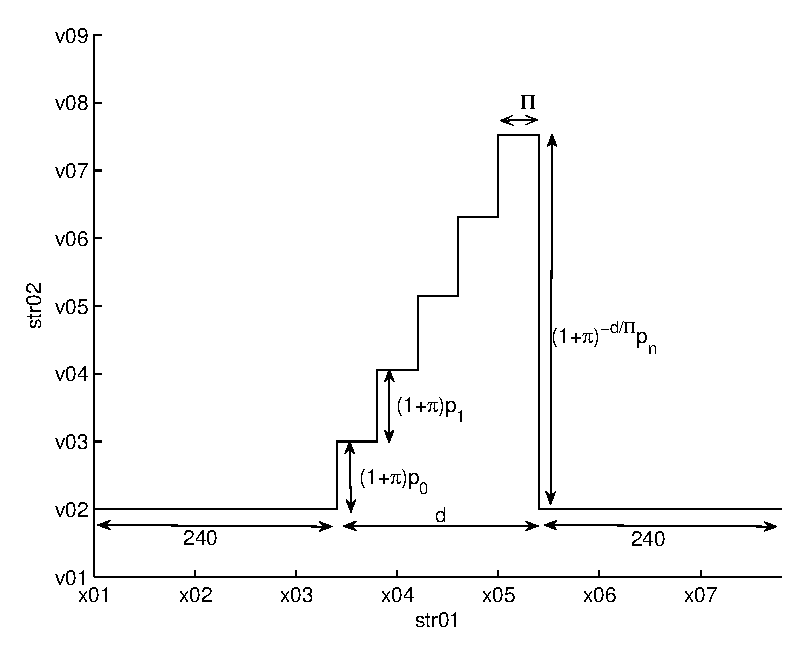
\epsfig{file=./energy_shock/eps/energy.eps}}%
\end{psfrags}%
%
% End energy.tex
\end{figure}\end{document}
% See http://www.uni-kassel.de/~linne/ for recent versions of laprint.m.
%
% created by:           LaPrint version 2.03 (19.1.2000)
% created on:           06-Oct-2009 10:58:03
% options used:         / noextrapicture
% latex width:          12 cm
% factor:               0.8
% eps file name:        energy.eps
% eps bounding box:     15 cm x 11.25 cm
% comment:              
%
\begin{psfrags}%
\psfragscanon%
%
% text strings:
\psfrag{str01}[t][t]{\sf Time (days)}%
\psfrag{str02}[t][t]{\sf Energy price}%
%
% xticklabels:
\psfrag{x01}[t][t]{0}%
\psfrag{x02}[t][t]{\sf 100}%
\psfrag{x03}[t][t]{\sf 200}%
\psfrag{x04}[t][t]{\sf 300}%
\psfrag{x05}[t][t]{\sf 400}%
\psfrag{x06}[t][t]{\sf 500}%
\psfrag{x07}[t][t]{\sf 600}%
%
% yticklabels:
\psfrag{v01}[r][r]{}%
\psfrag{v02}[r][r]{\sf $p_0$}%
\psfrag{v03}[r][r]{\sf $(1+\pi) p_0$}%
\psfrag{v04}[r][r]{\sf $(1+\pi)^2 p_0$}%
\psfrag{v05}[r][r]{}%
\psfrag{v06}[r][r]{}%
\psfrag{v07}[r][r]{}%
\psfrag{v08}[r][r]{}%
\psfrag{v09}[r][r]{}%
%
% Figure:
\resizebox{12cm}{!}{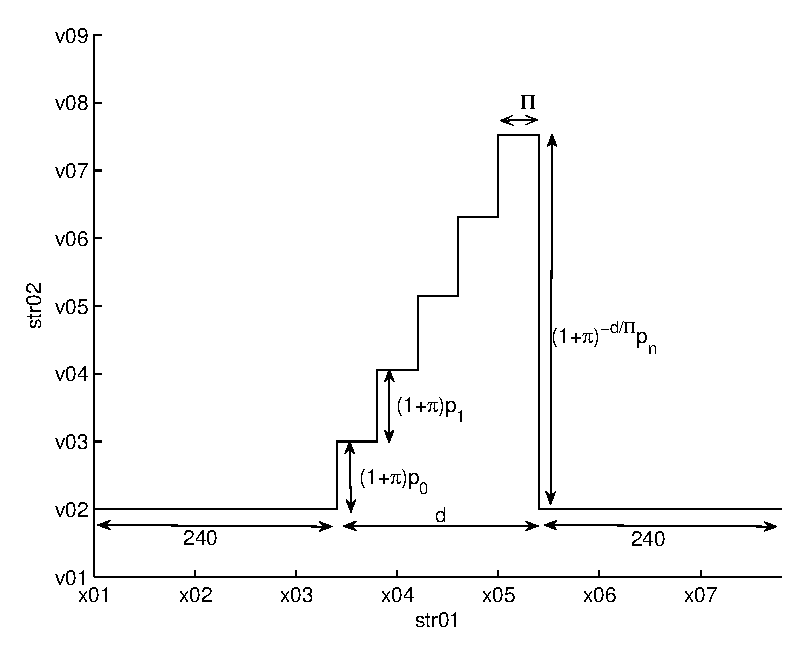
\epsfig{file=./energy_shock/eps/energy.eps}}%
\end{psfrags}%
%
% End energy.tex
\end{figure}\end{document}
% See http://www.uni-kassel.de/~linne/ for recent versions of laprint.m.
%
% created by:           LaPrint version 2.03 (19.1.2000)
% created on:           06-Oct-2009 10:58:03
% options used:         / noextrapicture
% latex width:          12 cm
% factor:               0.8
% eps file name:        energy.eps
% eps bounding box:     15 cm x 11.25 cm
% comment:              
%
\begin{psfrags}%
\psfragscanon%
%
% text strings:
\psfrag{str01}[t][t]{\sf Time (days)}%
\psfrag{str02}[t][t]{\sf Energy price}%
%
% xticklabels:
\psfrag{x01}[t][t]{0}%
\psfrag{x02}[t][t]{\sf 100}%
\psfrag{x03}[t][t]{\sf 200}%
\psfrag{x04}[t][t]{\sf 300}%
\psfrag{x05}[t][t]{\sf 400}%
\psfrag{x06}[t][t]{\sf 500}%
\psfrag{x07}[t][t]{\sf 600}%
%
% yticklabels:
\psfrag{v01}[r][r]{}%
\psfrag{v02}[r][r]{\sf $p_0$}%
\psfrag{v03}[r][r]{\sf $(1+\pi) p_0$}%
\psfrag{v04}[r][r]{\sf $(1+\pi)^2 p_0$}%
\psfrag{v05}[r][r]{}%
\psfrag{v06}[r][r]{}%
\psfrag{v07}[r][r]{}%
\psfrag{v08}[r][r]{}%
\psfrag{v09}[r][r]{}%
%
% Figure:
\resizebox{12cm}{!}{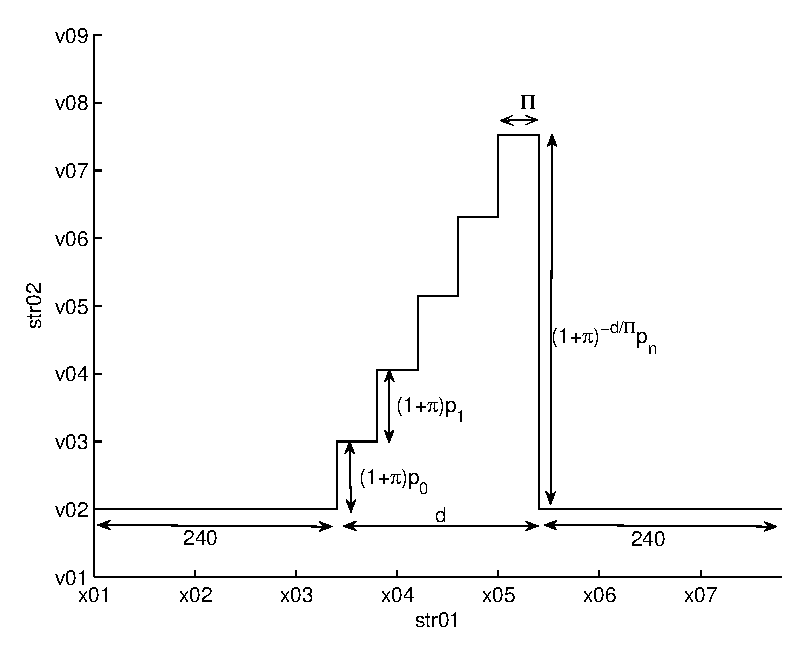
\epsfig{file=./energy_shock/eps/energy.eps}}%
\end{psfrags}%
%
% End energy.tex
